\documentclass[a4paper,11pt]{article}
\usepackage[utf8]{inputenc}
\usepackage[T1]{fontenc}
\usepackage[ngerman, english]{babel} % or remove ngerman if you only want English
\usepackage{geometry}
\usepackage{graphicx}
\usepackage{hyperref}
\usepackage{amsmath}
\usepackage{parskip}
\usepackage{enumitem}
\usepackage{booktabs}
\usepackage[ddmmyyyy]{isodate}
\usepackage{float}


\geometry{margin=1in}

\title{Exposé for Bachelor Thesis\\
\vspace{0.5em}
\large \textbf{Local LLM-Guided Robotic Control System for On-Demand Task Planning and Execution in Self-Driving Environments}\\
\vspace{2em}
\small
Technische Universität Berlin \\
Fakultät V - Verkehrs- und Maschinensysteme\\
Fachgebiet Industrielle Automatisierungstechnik
}

\author{
\textbf{Student:} Cemal Hekim, 500999 \\
B.Sc., Computational Engineering Science (Informationstechnik im Maschinenwesen) \vspace{1em} \\
\textbf{Supervisor:} Prof. Dr.-Ing. Jörg Krüger \\
\textbf{Secondary Supervisor:} Erik Sörqvist, M. Sc. \vspace{1em} \\
\textbf{External Contact:} Dr.-Ing. Özlem Özcan Sandikcioglu, \\ 
Bundesanstalt für Materialforschung und -prüfung, Division 6.2
}

\date{\today}

\begin{document}

\maketitle

\section{Motivation and Problem Statement}

The integration of AI technologies into industrial automation creates new opportunities for more flexible and user-friendly robotic control systems. Traditional robotic systems typically require complex programming or domain-specific expertise—such as proficiency in ROS 2, proprietary languages like ABB RAPID, or intermediate-level Python for API integration. This reliance on specialized skills limits their flexibility and usability, particularly in dynamic, semi-automated environments and for users without a technical background.

This thesis addresses these limitations by integrating a local Large Language Model (LLM) as a natural language interface to interpret user intent and autonomously plan and execute tasks. The project focuses on developing a control system where the LLM handles task planning based on user commands, executed through the uFactory xArm6 robotic arm. Real-world tasks such as measurements will demonstrate the system’s capability, and development will take place in BAM’s autonomous laboratory to ensure technical and practical relevance.

\section{State of Research}

Recent research has explored using Large Language Models (LLMs) for task planning in robotics. Studies like DELTA \cite{liu2024delta} and LLM as BT-Planner \cite{ao2024llm} demonstrate how LLMs can generate adaptable behavior trees for complex tasks. Additionally, RoboChat \cite{10489289} presents an interactive framework for controlling mobile robots using LLMs. Despite these advances, LLMs' application for real-time robot control in industrial and laboratory automation remains underexplored, suggesting a need for further research.

\newpage

\section{Objectives}

The main objectives of this thesis are:

\begin{itemize}
    \item Investigate the use of Large Language Models (LLMs) for task planning in robotic control systems, focusing on the translation of natural language inputs into executable commands.
    
    \item Implement a system where a local LLM processes user commands and translates them into structured function calls. 
    
    \item Integrate the system with the uFactory xArm6 robotic arm using its Python API or ROS2 interface. Pre-define functions from robot's framework for LLM to perform tasks, such as:
    \begin{verbatim}
move_to(location="A")
activate_gripper(action="close")
measure.palmsens(measurement_data="X")
    \end{verbatim}

    \item Ensure the system can perform precise tasks like pick-and-place and reconfiguration.
    
    \item (Optional Demonstration Case \#1) Develop a real-time application for lab automation, specifically for electrochemical measurements. The system will execute tasks based on user commands, such as:
    \begin{quote}
        \textit{“Pick up the sample X, place it in station B, and start testing A value.”}
    \end{quote}
    
    \item Evaluate the system’s performance in various scenarios, looking at accuracy, speed, error handling, and user interaction.
    
    \item Compare the system with existing robotic control solutions based on performance, focusing on flexibility, ease of use, and adaptability.
    
    \item (Future) Explore adding voice and visual input as a goal, using speech-to-text to get the user input and image recognition for perception and SLAM to execute the tasks. These features may be developed further in the next semester.
\end{itemize}

\newpage

\section{Methodology}

The project will be developed through the following steps:
\begin{itemize}
    \item \textbf{System Architecture Design:} The system will consist of three components: a natural language input module using a local LLM, a task translation layer that maps LLM outputs to robot control functions, and the robot control interface connected to the uFactory xArm6.

    \begin{figure}[H]
        \centering
        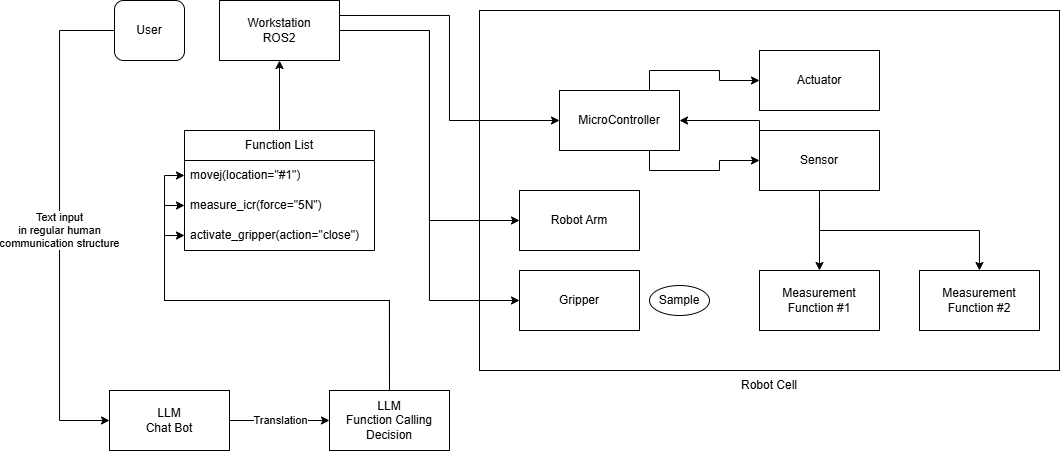
\includegraphics[width=1\linewidth]{images/flow.drawio (1).png}
        \caption{System architecture flow diagram including the measurement setup necessary for the Lab-Automation use case}
        \label{fig:system-architecture}
    \end{figure}
    
    \item \textbf{LLM Prompt Setup:} The local LLM will be set up to generate structured robot commands. Prompt templates and examples will be used. 
    
    \item \textbf{Task Translation Layer:} A parser will be implemented to convert the LLM's output into direct Python function calls compatible with the robot's API or ROS2 services.
    
    \item \textbf{Robot Control Module:} Pre-defined functions will be created for robot movements, inverse kinematics, and gripper actions. The module will provide a callable interface for executing tasks.
    
    \item \textbf{System Integration:} The LLM, task parser, and robot control module will be combined into a single application. Simple asynchronous messaging will be used between modules if needed.
    
    \item \textbf{Testing:} Unit tests for each module will be performed first, followed by tests on the complete system using basic task sequences.
    
    \item \textbf{Scenario Testing:} The system will be tested on tasks like pick-and-place, sample repositioning, and simple lab measurements. Behavior will be checked for different types of user inputs (correct, ambiguous, incorrect).
    
    \item \textbf{Performance Measurement:} Metrics such as command accuracy, task completion time, error rates, and system stability will be recorded and compared to baseline manual control.
\end{itemize}

\newpage
\section{Strengths and Deliverables}

The main strengths of the project are:

\begin{itemize}
    \item Direct robot control from natural language without manual coding.
    \item Local LLM for offline operation, ensuring data privacy and reliability.
    \item Modular system design: independent language processing, task translation, and robot control.
    \item Designed for real-time responsiveness in industrial, warehouse, and laboratory environments.
\end{itemize}

The expected deliverables are the following.

\begin{itemize}
    \item Local application for natural language-based robot control.
    \item Task translation module mapping LLM output to robot API calls or ROS2 subscribers.
    \item Robot control module including movement, gripper control, and basic error handling.
    \item System documentation (architecture, setup, usage, extension guide).
    \item Performance evaluation report (accuracy, speed, error rates).
    \item User feedback report from both expert and non-expert participants to evaluate system usability and accessibility.

\end{itemize}

\section{Work Plan and Timeline}

\begin{tabular}{|p{0.3\linewidth}|p{0.6\linewidth}|}
\hline
\textbf{Phase} & \textbf{Description} \\
\hline
01.07.2025 – 31.07.2025 & Preparations for the Thesis \\
25.07.2025 & The Last Exam Day in SoSe25 \\
01.08.2025 & Potential Start Date of the Thesis \\
01.10.2025 & Start Date of WiSe25-26 (1st Master Semester) \\
15.10.2025 & Start Date of the Project Modul at FG IAT \\
31.10.2025 & Potential Submission Date for Thesis \\
31.03.2026 & End Date of the Project Modul at FG IAT \\
\hline
\end{tabular}

\begin{figure}[H]
    \centering
    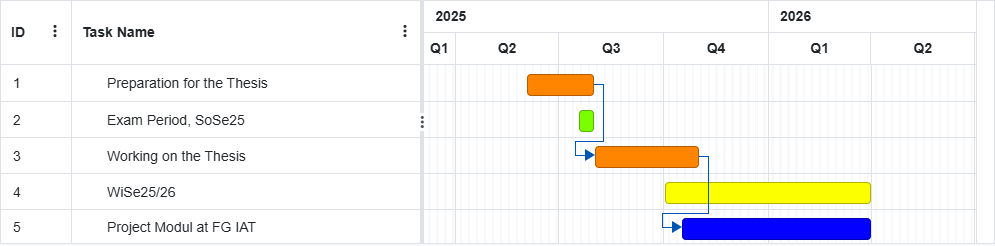
\includegraphics[width=1.0\linewidth]{images/Online Gantt 20250428 (3).png}
    \caption{Gantt Chart of the Timeline}
    \label{fig:enter-label}
\end{figure}

\vspace{1em}
\textit{The development of the project can be continued at the Modul, Automatisierungstechnisches Projekt, with applications in Medical Use during WiSe2025-2026.}

\newpage
\begin{thebibliography}{9}
\bibitem{liu2024delta} Yuchen Liu et al., "DELTA: Decomposed Efficient Long-Term Robot Task Planning using Large Language Models," arXiv:2404.03275, 2024. \url{https://arxiv.org/abs/2404.03275}

\bibitem{ao2024llm} Jicong Ao et al., "LLM as BT-Planner: Leveraging LLMs for Behavior Tree Generation in Robot Task Planning," arXiv:2409.10444, 2024. \url{https://arxiv.org/abs/2409.10444}

\bibitem{10489289} Guang Li et al., "RoboChat: A Unified LLM-Based Interactive Framework for Robotic Systems," in \textit{2023 5th International Conference on Robotics, Intelligent Control and Artificial Intelligence (RICAI)}, 2023, pp. 466-471. DOI: \url{10.1109/RICAI60863.2023.10489289}


\end{thebibliography}


\end{document}
